% !TeX program = xelatex
\documentclass[a4paper,12pt]{article}
\usepackage{graphicx}
\usepackage{amsmath}
\usepackage{here}
\usepackage{geometry}
\geometry{margin=25mm}

% 日本語の表示に必要なパッケージとフォント設定
\usepackage{xeCJK}
\setCJKmainfont{Noto Sans CJK JP}
\usepackage{fontspec}
\setsansfont{Noto Sans CJK JP}
\setmonofont{Noto Sans Mono CJK JP}

\begin{document}

\title{センサ工学 Home Work 1}
\author{21C1002 相田 舟星}
\date{}
\maketitle

\section*{問題1}

\begin{itemize}
    \item $N(0, 1)$:平均 $\mu=0$, 標準偏差 $\sigma=1$
    \item $N(0, 4)$:平均 $\mu=0$, 標準偏差 $\sigma=2$
    \item $N(0, 9)$:平均 $\mu=0$, 標準偏差 $\sigma=3$
    \item $N(4, 4)$:平均 $\mu=4$, 標準偏差 $\sigma=2$
\end{itemize}

各分布の曲線は、平均値の $\pm3\sigma$ の範囲を含むようにプロット。

\begin{figure}[H]
    \centering
    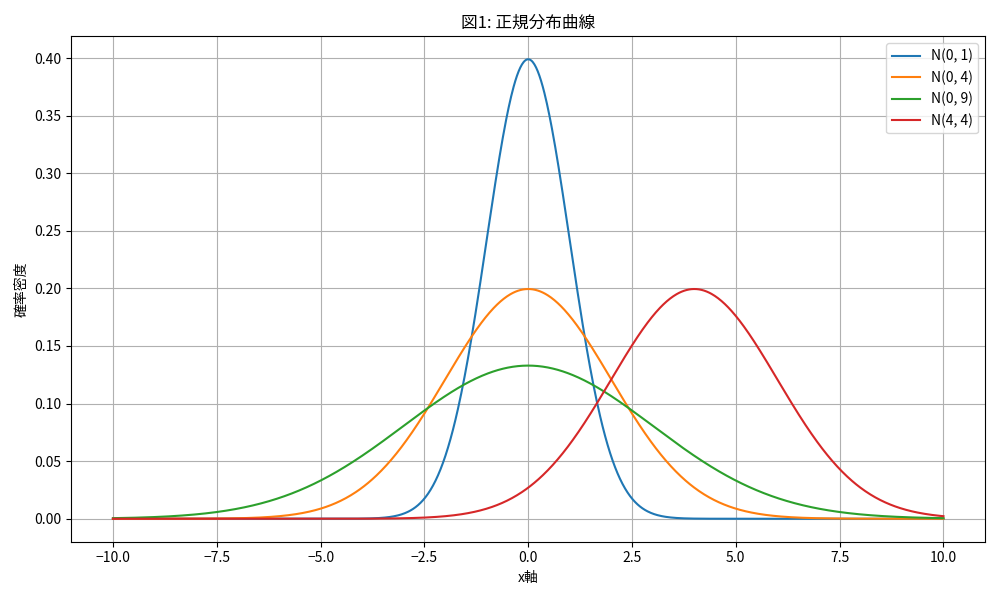
\includegraphics[width=0.8\textwidth]{Figure_1.png}
    \caption{正規分布 $N(0, 1)$、$N(0, 4)$、$N(0, 9)$、$N(4, 4)$ の確率分布曲線}
\end{figure}

\section*{問題2}

学籍番号の下2桁が「02」なので、$StdID = 2$ と設定。

\begin{itemize}
    \item $N(0, 1)$:平均 $\mu=0$, 標準偏差 $\sigma=1$
    \item $N(2, 4)$:平均 $\mu=2$, 標準偏差 $\sigma=2$
\end{itemize}

各分布の曲線は、平均値の $\pm3\sigma$ の範囲を含むようにプロット。

\begin{figure}[H]
    \centering
    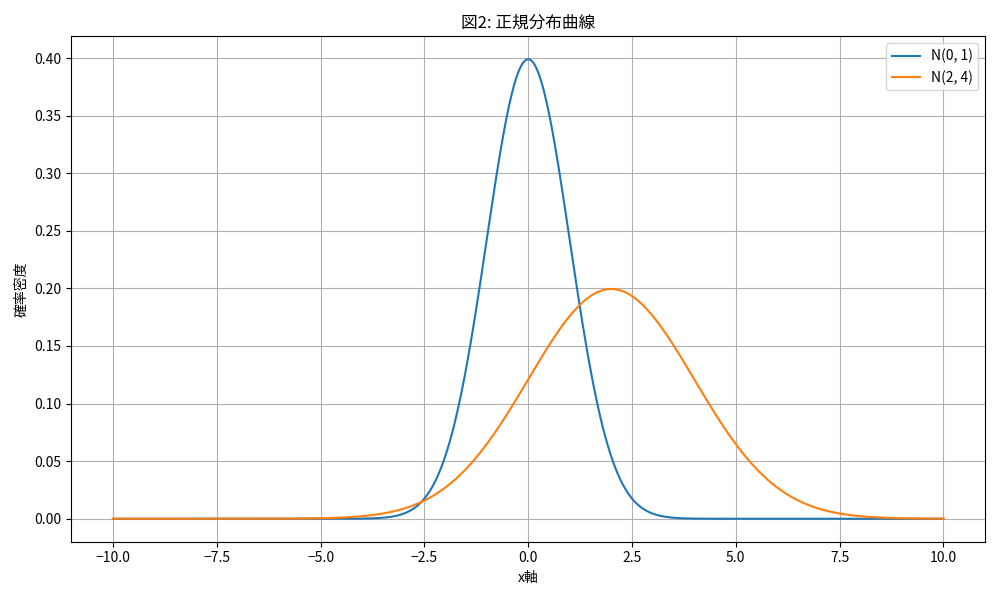
\includegraphics[width=0.8\textwidth]{Figure_2.png}
    \caption{正規分布 $N(0, 1)$ と $N(2, 4)$ の確率分布曲線}
\end{figure}

\section*{問題3}

\subsection*{回路 (a)}

\begin{itemize}
    \item 抵抗 $R_1$ にかかる電圧:$U_1 = 3.1\,\mathrm{V}$
    \item 抵抗 $R_2$ にかかる電圧:$U_2 = 0.55\,\mathrm{V}$
\end{itemize}

全体の電圧 $U$ は各電圧の和。

\[
U = U_1 + U_2 = 3.1\,\mathrm{V} + 0.55\,\mathrm{V} = 3.65\,\mathrm{V}
\]

有効数字と丸め誤差を考慮し、小数点以下1桁までとする。

\[
U = 3.65\,\mathrm{V} \approx 3.7\,\mathrm{V}
\]

したがって、全体の電圧 $U$ は $3.7\,\mathrm{V}$。

\subsection*{回路 (b)}

\begin{itemize}
    \item 抵抗 $R_1 = 5\,\mathrm{k\Omega}$
    \item 抵抗 $R_2 = 0.33\,\mathrm{k\Omega}$
    \item 電流 $I = 10\,\mathrm{mA}$
\end{itemize}

総抵抗は次のように計算。

\[
R = R_1 + R_2 = 5\,\mathrm{k\Omega} + 0.33\,\mathrm{k\Omega} = 5.33\,\mathrm{k\Omega}
\]

有効数字を考慮し、小数点以下0桁までとする。

\[
R = 5.33\,\mathrm{k\Omega} \approx 5\,\mathrm{k\Omega}
\]

オームの法則より全体の電圧 $U$ は

\[
U = I \times R = 10\,\mathrm{mA} \times 5\,\mathrm{k\Omega} = 50\,\mathrm{V}
\]

したがって、全体の電圧 $U$ は $50\,\mathrm{V}$。

\section*{Ex.1}

正規分布 $N(\mu, \sigma^2)$ の確率密度関数は

\[
f(x) = \frac{1}{\sigma \sqrt{2\pi}} \exp\left( -\frac{(x - \mu)^2}{2\sigma^2} \right)
\]

$x$ が範囲 $[\mu - 3\sigma,\, \mu + 3\sigma]$ に含まれる確率は

\[
P(\mu - 3\sigma \leq x \leq \mu + 3\sigma) = \int_{\mu - 3\sigma}^{\mu + 3\sigma} f(x)\,dx
\]

標準化変数 $z$ を用いて変数変換を行う。

\[
z = \frac{x - \mu}{\sigma}
\]

これにより、確率は

\[
P(-3 \leq z \leq 3) = \int_{-3}^{3} \frac{1}{\sqrt{2\pi}} \exp\left( -\frac{z^2}{2} \right)\,dz
\]

標準正規分布表または数値計算により

\[
\Phi(3) \approx 0.99865,\quad \Phi(-3) \approx 0.00135
\]

したがって、

\[
P(-3 \leq z \leq 3) = \Phi(3) - \Phi(-3) = 0.99865 - 0.00135 = 0.9973
\]

パーセンテージで表すと

\[
0.9973 \times 100\% = 99.73\%
\]

よって、$x = \mu \pm 3\sigma$ の範囲に含まれる確率は約99.7\%。

\end{document}
